\chapter[Техническое обслуживание]{Техническое обслуживание и устранение неисправностей}
\label{chap:maintenance_and_troubleshooting}

\section{Обновление прошивки}

\warningbox{
  Прочтите, прежде чем приступать к работе В результате обновления
  прошивки могут быть потеряны калибровочные константы
  в вашем гравиметре \cg{}. Убедитесь, что у вас есть резервная копия этих
  констант.

  В ходе обновления питание гравиметра \cg{} должно быть бесперебойным.
}

\subsection{Что нужно для обновления прошивки}

\begin{itemize}
  \item Гравиметр \cg{}

  \item Штатный планшет со средой Windows или любой ПК со средой Windows с
    функцией Bluetooth.

  \item Файл hex новой версии прошивки CG-6

  \item LynxLG~-- программное обеспечение для обработки данных наземной
    гравиметрии (предварительно установленное в штатный планшет под Windows),
    или Программа обновления прошивки CG-6,
    загруженная с
    \url{https://scintrexltd.com/support/product-software-updates/}
\end{itemize}

\subsection{Подготовка к обновлению прошивки}
\label{subsec:preparing_to_upgrade_your_firmware}

Чтобы провести обновление прошивки, нужно установить
соединение по Bluetooth между вашим гравиметром \cg{} и планшетом или ПК.

\infobox{
  Настоящее руководство подготовлено для среды Windows~7. Если вы пользуетесь
  другой версией операционной системы Windows, интерфейсы могут отличаться.
}

Щёлкните мышкой на графическом символе Bluetooth \faBluetooth{} на панели задач.
Выберите в меню пункт <<Add a Device>>, как показано ниже.

\begin{figure}[H]
  \centering
  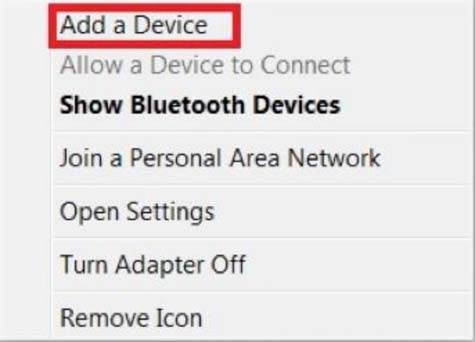
\includegraphics[width=0.4\textwidth]{figures/adding_a_bluetooth_device}
  \caption{Добавление устройства Bluetooth}
  \label{fig:adding_a_bluetooth_device}
\end{figure}

В качестве альтернативы, вы можете найти команду <<Add a Bluetooth device>> на
Панели управления.

\begin{figure}[H]
  \centering
  
\includegraphics[width=0.8\textwidth]{figures/adding_a_bluetooth_device_from_the_control_panel}
  \caption{Добавление устройства Bluetooth с Панели управления}
  \label{fig:adding_a_bluetooth_device_from_the_control_panel}
\end{figure}

Выберите из списка устройств гравиметр CG-6 и щёлкните на кнопке <<Next>>

\newpage
\begin{figure}[H]
  \centering
  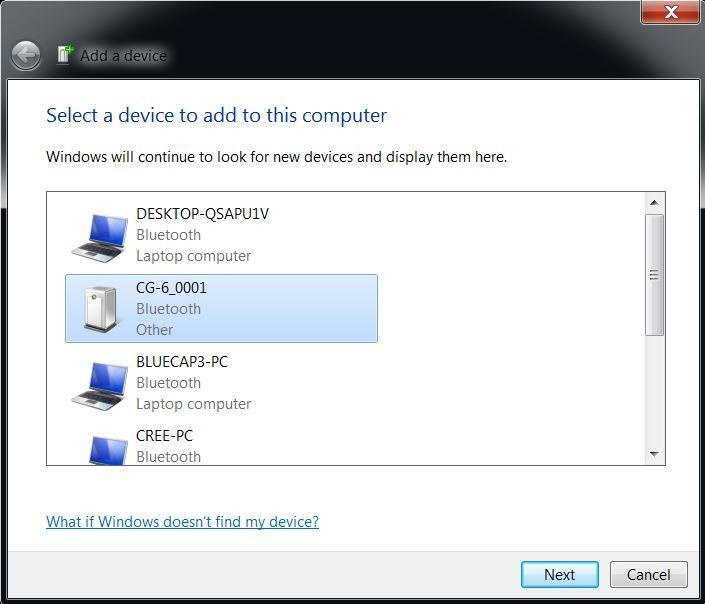
\includegraphics[width=0.6\textwidth]{figures/selecting_a_bluetooth_device}
  \caption{Выбор устройства Bluetooth}
  \label{fig:selecting_a_bluetooth_device}
\end{figure}

После того, как ваш гравиметр \cg{} будет успешно добавлен к списку устройств
Bluetooth, вы увидите показанное ниже экранное изображение.  Щёлкните мышкой на
кнопке <<Close>>.

\begin{figure}[H]
  \centering
  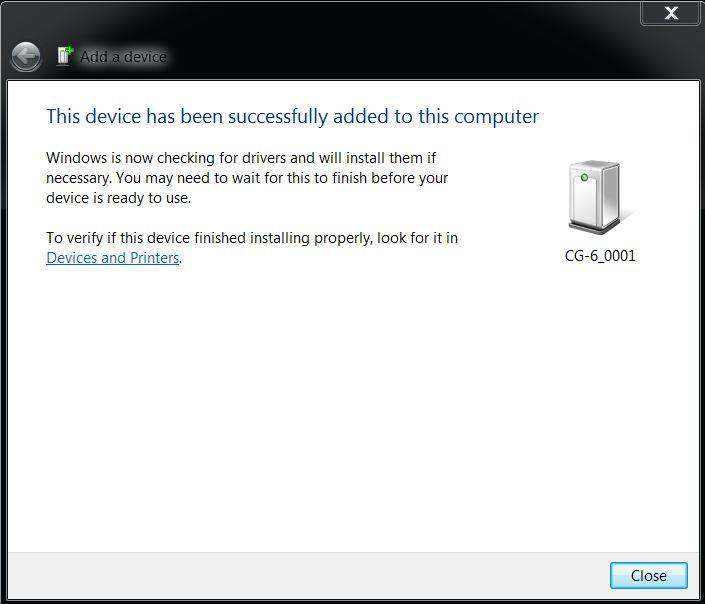
\includegraphics[width=0.6\textwidth]{figures/bluetooth_device_successfully_added}
  \caption{Устройство Bluetooth успешно добавлено}
  \label{fig:bluetooth_device_successfully_added}
\end{figure}

Щёлкните мышкой на пункте <<Show Bluetooth Devices>> в меню Bluetooth, и вы
увидите гравиметр \cg{} в списке устройств. Щёлкните правой кнопкой мышки на
графическом символе CG-6, и выделите пункт <<Properties>>.

\begin{figure}[H]
  \centering
  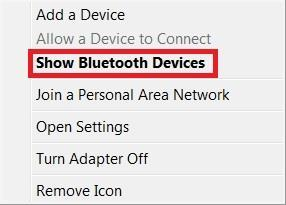
\includegraphics[width=0.4\textwidth]{figures/bluetooth_device_properties}
  \caption{Свойства устройства Bluetooth}
  \label{fig:bluetooth_device_properties}
\end{figure}

\infobox{
  Четыре цифры после наименования CG-6~-- это порядковый номер вашего
  устройства, который будет отличаться от 0001.
}

На странице под закладкой <<Hardware>> найдите номер COM-порта (в данном примере
это COM3). Запишите номер этого COM-порта для использования в последующих
действиях.

\newpage
\begin{figure}[H]
  \centering
  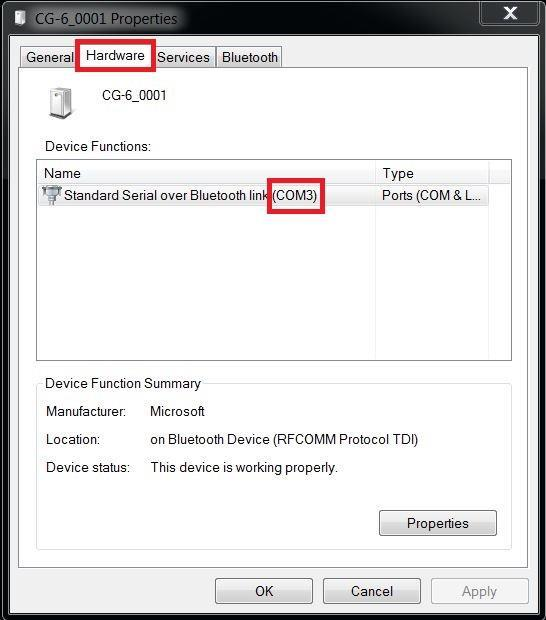
\includegraphics[width=0.6\textwidth]{figures/bluetooth_device_com_port}
  \caption{COM-порт для устройства Bluetooth}
  \label{fig:bluetooth_device_com_port}
\end{figure}

\subsection[Обновление прошивки при помощи LynxLG]{Обновление прошивки обеспечения CG-6 при помощи программы LynxLG}
\label{subsec:upgrading_cg6_firmware_with_lynxlg_software}

\infobox{
  Если у вас нет доступа к программе обработки данных наземной гравиметрии
  LynxLG, переходите к следующему разделу, который называется
  \nameref{subsec:upgrade_the_cg6_firmware_with_cg6_firmware_updater_software}
}

\subsubsection{Создайте резервные копии калибровочных констант}

Запустите программу LynxLG. Щёлкните мышкой на кнопке <<Settings>> на главном
экранном изображении.

\newpage
\begin{figure}[H]
  \centering
  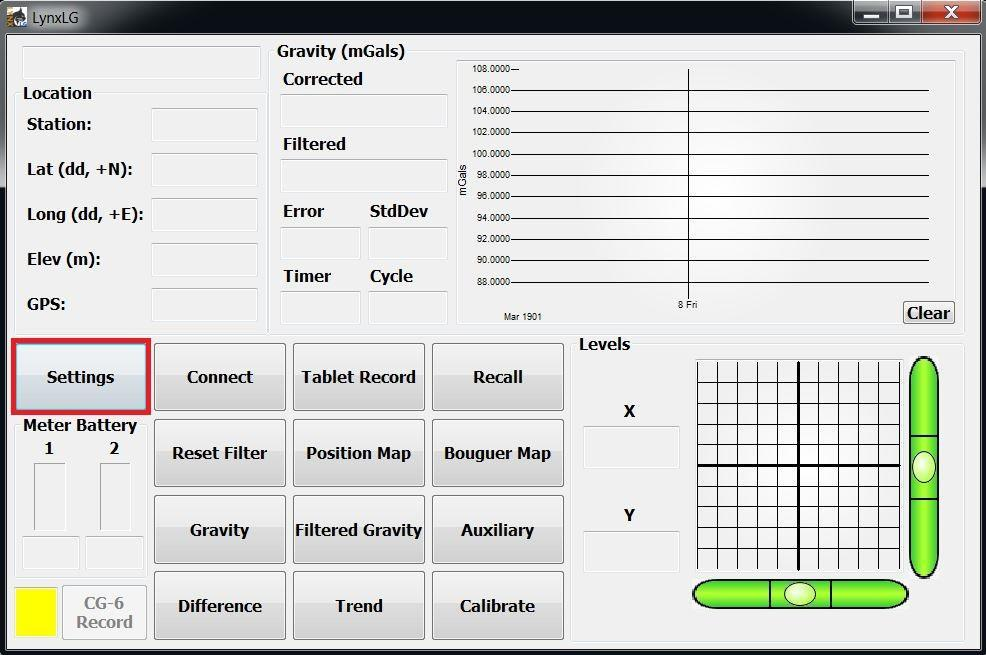
\includegraphics[width=0.7\textwidth]{figures/the_lynxlg_software_main_screen}
  \caption{Главное экранное изображение программы LynxLG}
  \label{fig:the_lynxlg_software_main_screen}
\end{figure}

Перейдите на страницу под закладкой <<Calibration>> и щёлкните мышкой на кнопке
<<Get/Set Factors>>.

\begin{figure}[H]
  \centering
  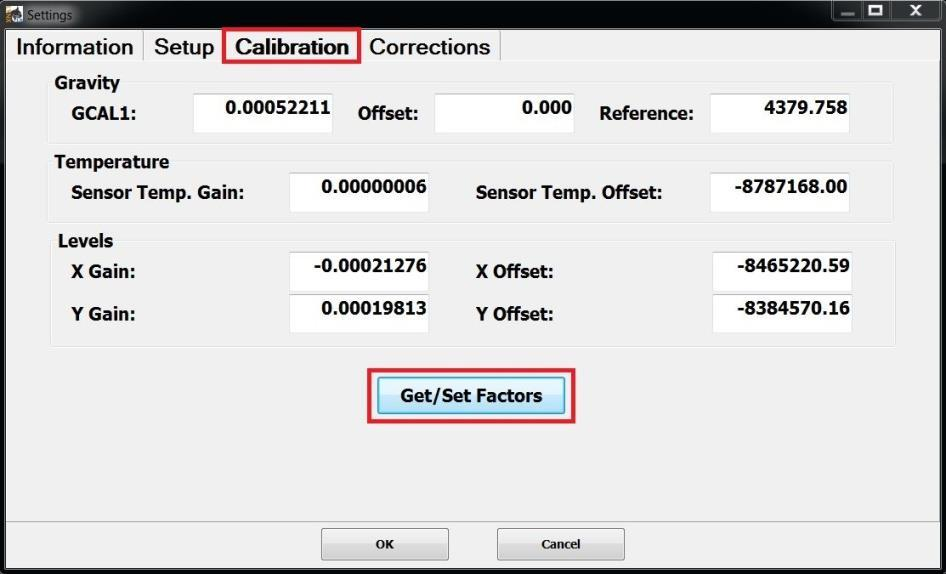
\includegraphics[width=0.7\textwidth]{figures/the_lynxlg_software_calibration_screen}
  \caption{Экран калибровки программы LynxLG}
  \label{fig:the_lynxlg_software_calibration_screen}
\end{figure}

Щёлкните мышкой на кнопках <<Get>>, чтобы синхронизировать калибровочные
константы гравиметра CG-6 с LynxLG, как показано ниже. Для сохранения этих
изменений щёлкните мышкой на кнопке <<OK>>.

\begin{figure}[H]
  \centering
  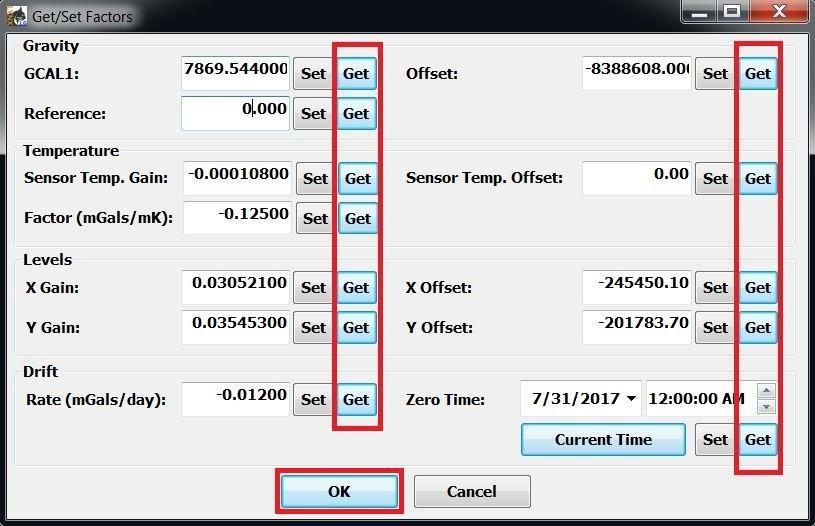
\includegraphics[width=0.7\textwidth]{figures/the_lynxlg_software_get_set_factors_screen}
  \caption{Экранное изображение «Get/Set Factors» в программе LynxLG}
  \label{fig:the_lynxlg_software_get_set_factors_screen}
\end{figure}

\subsubsection{Обновление прошивки}
\label{subsubsec:update_firmware}

Вернитесь в главное экранное изображение программы LynxLG, как показано ниже.
Щёлкните мышкой на графическом символе LynxLG в верхнем левом углу, и в
раскрывшемся меню выделите пункт <<Upgrade Firmware>>.

\begin{figure}[H]
  \centering
  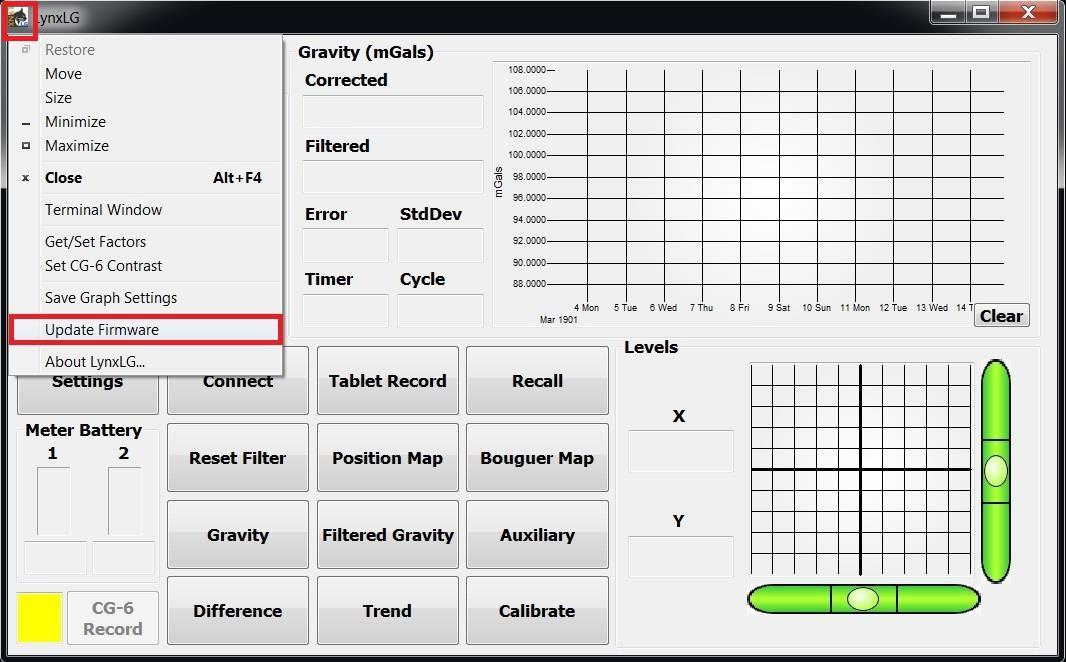
\includegraphics[width=0.7\textwidth]{figures/update_firmware_pull-down_menu}
  \caption{Меню обновления прошивки}
  \label{fig:update_firmware_pull-down_menu}
\end{figure}

В следующих двух окнах сообщений, показанных ниже, щёлкните мышкой на
кнопках <<Yes>> и <<OK>>.

\begin{figure}[H]
  \centering
  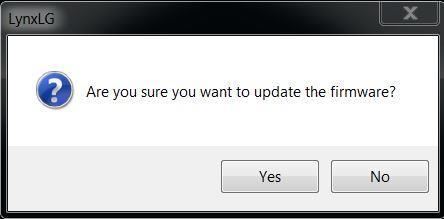
\includegraphics[width=0.4\textwidth]{figures/confirming_the_firmware_update_1}
  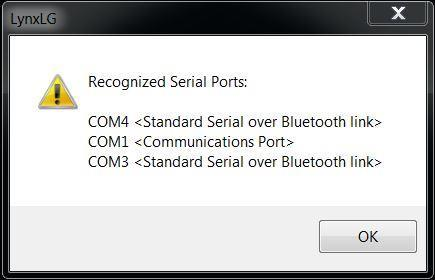
\includegraphics[width=0.4\textwidth]{figures/confirming_the_firmware_update_2}
  \caption{Подтверждение обновления прошивки}
  \label{fig:confirming_the_firmware_update}
\end{figure}

Произведите настройку портов, как показано ниже. Используйте COM-порт
присвоенный гравиметру \cg{} (если имеются неясности, обратитесь к разделу
\nameref{subsec:preparing_to_upgrade_your_firmware}). Параметр Baud Rate
(Скорость передачи) нужно задать равным 115200, Data Bits (Информационные
биты)~-- равным 8, Parity (Контроль чётности)~-- None, и Stop Bit (Стоповый
бит)~-- задать равным 1. Щёлкните мышкой на кнопке <<OK>>.

\begin{figure}[H]
  \centering
  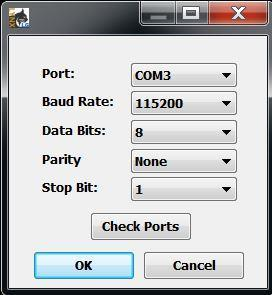
\includegraphics[width=0.4\textwidth]{figures/com_port_configuration}
  \caption{Конфигурация COM-портов}
  \label{fig:com_port_configuration}
\end{figure}

Сейчас ваш гравиметр \cg{} готов войти в \textbf{режим обновления прошивки}, как
показано ниже.

\begin{figure}[H]
  \centering
  
\includegraphics[width=0.4\textwidth]{figures/the_cg6_in_upgrade_mode}
  \caption{Гравиметр CG-6 в режиме обновления}
  \label{fig:the_cg6_in_upgrade_mode}
\end{figure}

\warningbox{
  Если обновление окажется неуспешным и ваш гравиметр \cg{} зависнет с показанной
  выше картинкой на экране, произведите цикл выключения/включения питания
  (отсоедините и вновь присоедините все аккумуляторные батареи, а также шнур
  электропитания). После этого гравиметр \cg{} должен включиться обычным образом.
}

В программе LynxLG вы увидите показанное ниже экранное изображение. Убедитесь,
что вы выбрали нужный COM-порт и правильно задали скорость передачи данных.
Щёлкните мышкой на кнопке <<Connect>>.

\begin{figure}[H]
  \centering
  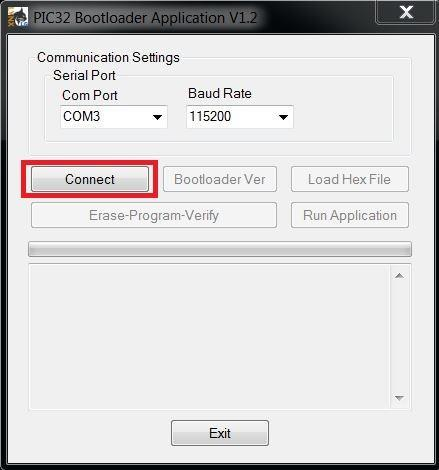
\includegraphics[width=0.49\textwidth]{figures/connecting_the_cg6_with_lynxlg_bootloader}
  \caption{Установление соединения прибора CG-6 с LynxLG Bootloader}
  \label{fig:connecting_the_cg6_with_lynxlg_bootloader}
\end{figure}

После успешного установления соединения щёлкните мышкой на кнопке <<Load Hex
File>>, как показано ниже.

\begin{figure}[H]
  \centering
  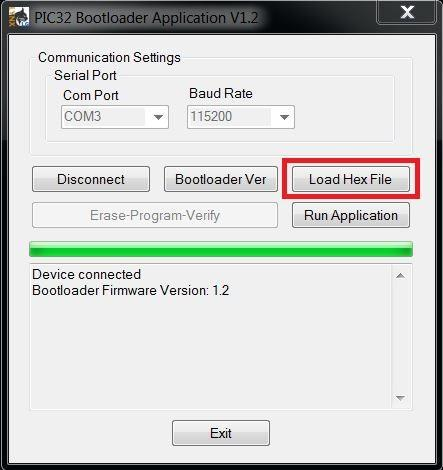
\includegraphics[width=0.49\textwidth]{figures/loading_the_hex_file_with_lynxlg_bootloader}
  \caption{Загрузка файла hex с помощью LynxLG Bootloader}
  \label{fig:loading_the_hex_file_with_lynxlg_bootloader}
\end{figure}

Выделите файл *.hex, который вы хотели бы применить, как показано ниже.

\begin{figure}[H]
  \centering
  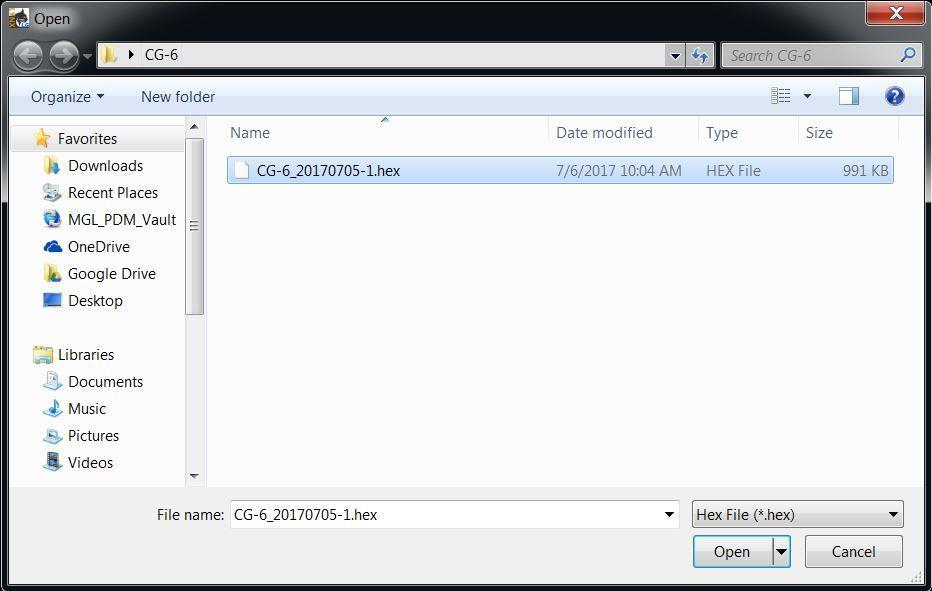
\includegraphics[width=0.7\textwidth]{figures/selecting_the_hex_file_with_the_lynxlg_bootloader}
  \caption{Выделение файла hex с помощью LynxLG Bootloader}
  \label{fig:selecting_the_hex_file_with_the_lynxlg_bootloader}
\end{figure}

После загрузки файла hex, щёлкните мышкой на кнопке <<Erase-Program-Verify>>,
как показано ниже.

\begin{figure}[H]
  \centering
  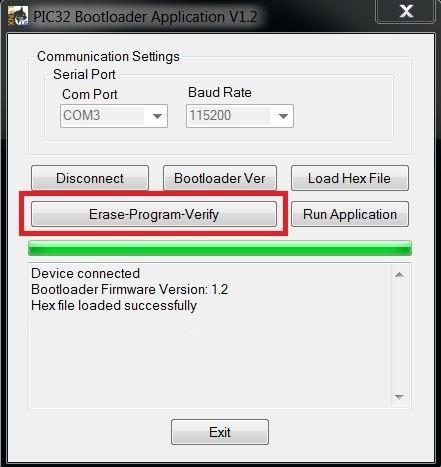
\includegraphics[width=0.49\textwidth]{figures/verifying_the_program_with_the_lynxlg_bootloader}
  \caption{Проверка программы при помощи LynxLG Bootloader}
  \label{fig:verifying_the_program_with_the_lynxlg_bootloader}
\end{figure}

Дождитесь успешного завершения стирания, программирования и проверки (это может
занять несколько минут). После этого щёлкните мышкой на кнопке <<Run
Application>>, как показано ниже.

\newpage
\begin{figure}[H]
  \centering
  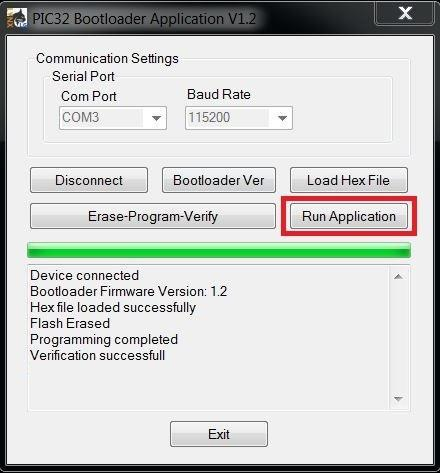
\includegraphics[width=0.49\textwidth]{figures/upgrade_firmware_with_lynxlg_bootloader}
  \caption{Прошивка обновлена с помощью LynxLG Bootloader}
  \label{fig:upgrade_firmware_with_lynxlg_bootloader}
\end{figure}

Ваш гравиметр \cg{} должен выйти из режима обновления прошивки и запустить его новую версию.

\subsubsection{Восстановление калибровочных констант}

Вернитесь к экранному изображению Settings/Calibration Tab/Get/Set Factors, как
показано ниже. Щёлкните мышкой на всех кнопках <<Set>> для синхронизации всех
калибровочных констант из LynxLG обратно в ваш гравиметр \cg{}.

\newpage
\begin{figure}[H]
  \centering
  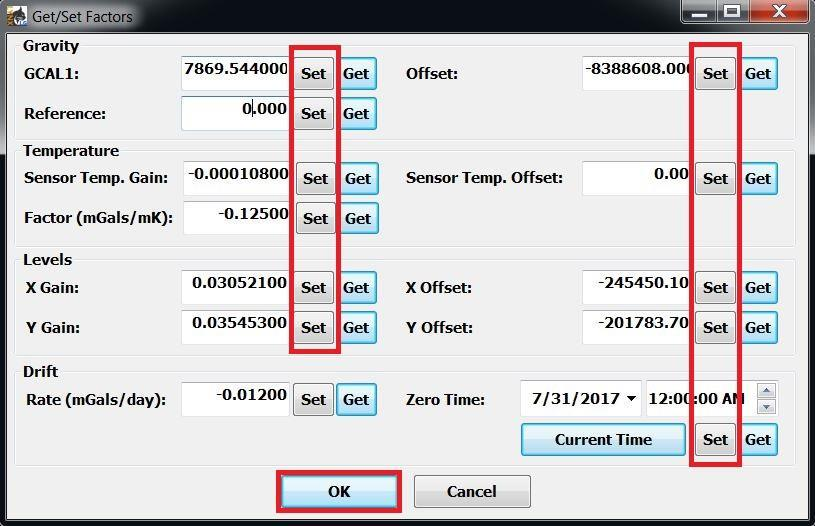
\includegraphics[width=0.7\textwidth]{figures/the_lynxlg_sortware_get_set_factors_screen}
  \caption{Экранное изображение «Get/Set Factors» в программе LynxLG}
  \label{fig:the_lynxlg_sortware_get_set_factors_screen}
\end{figure}

\infobox{
  Все иллюстрации выше показаны в качестве примера. Константы вашего гравиметра
  \cg{} будут другими.
}

\subsection[Обновление прошивки с помощью программы обновления]{Обновление
  прошивки CG-6 с помощью программы обновления}
\label{subsec:upgrade_the_cg6_firmware_with_cg6_firmware_updater_software}

\subsubsection{Создайте резервные копии калибровочных констант}

Перейдите к экранному изображению <<SETTINGS/CALIB>> (см. ниже) на вашем
гравиметре \cg{}. Выпишите значения всех калибровочных констант.  Вы можете
сохранить их в текстовом файле, записать на бумаге, или просто сделать снимок
экрана.

\begin{figure}[H]
  \centering
  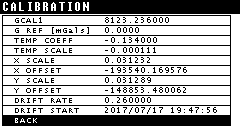
\includegraphics[width=0.49\textwidth]{figures/the_cg6_calibration_screen}
  \caption{Экранное изображение калибровки CG-6}
  \label{fig:the_cg6_calibration_screen_2}
\end{figure}

\subsubsection{Загрузите и установите программу обновления
  прошивки CG-6}

Пройдите по следующей ссылке, откуда можно загрузить программу обновления
прошивки CG-6:
\url{https://scintrexltd.com/support/product-software-updates/}

Запустите программу установки и следуйте указаниям на экране.

\subsubsection{Обновление прошивки}

Запустите программу обновления прошивки CG-6. Она имеет такой же интерфейс, что
и встроенные функциональные средства обновления прошивки в LynxLG. Обратитесь к
параграфу \nameref{subsubsec:update_firmware} в разделе
\nameref{subsec:upgrading_cg6_firmware_with_lynxlg_software}.

\begin{figure}[H]
  \centering
  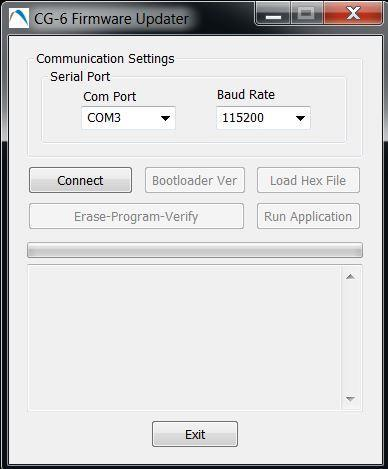
\includegraphics[width=0.49\textwidth]{figures/cg6_firmware_update_main_screen}
  \caption{Главный экран программы обновления прошивки CG-6}
  \label{fig:cg6_firmware_update_main_screen}
\end{figure}

\subsubsection{Восстановление калибровочных констант}

Перейдите к экранному изображению <<SETTINGS/CALIB>> (см. ниже) на вашем
гравиметре \cg{}. Отредактируйте каждую запись в соответствии с ранее записанными
значениями.

\begin{figure}[H]
  \centering
  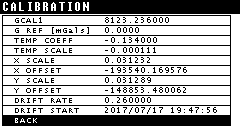
\includegraphics[width=0.49\textwidth]{figures/the_cg6_calibration_screen}
  \caption{Экранное изображение калибровки CG-6}
  \label{fig:the_cg6_calibration_screen}
\end{figure}

\infobox{
  Все иллюстрации показаны выше в качестве примера.  Константы вашего гравиметра
  \cg{} будут другими.
}

\section{Поиск и устранение неисправностей}

\warningbox{
  При обращении с гравиметром \cg{} необходимо соблюдать осторожность. Нужно
  избегать сильных толчков и ударов.
}

Несмотря на то, что прибор \cg{} характеризуется высокой надёжностью, в некоторых
обстоятельствах вы можете столкнуться с неполадками. В представленной ниже
таблице содержится список некоторых проблем и способов их решения. Тем не менее,
в случае необходимости обращайтесь к нам безо всяких колебаний. Контактная
информация содержится в разделе <<Гарантия и ремонт>>.

\begin{longtable}{|p{0.25\textwidth}|p{0.25\textwidth}|p{0.4\textwidth}|}
  \hline
  Проблема & Возможная причина & Возможное решение \\
  \hline
  \cg{} не включается &
  Разряжена аккумуляторная батарея или прибор не подключён к сети переменного
  тока. & 
  Подключите источник питания (No 128370015) и/или установите полностью
  заряженную аккумуляторную батарею. \\
  \cline{2-3}
  & Аккумуляторная батарея не до конца вставлена в прибор. &
  С усилием, но соблюдая осторожность, надавите на крышку каждой из
  аккумуляторных батарей. \\
  \hline
  Заряд и разряд аккумуляторной батареи происходит с отклонением от нормы,
  например, батарея, заряжается быстрее, чем обычно, но её ёмкость ниже нормы. &
  Утрачена калибровка аккумуляторной батареи. &
  Вставьте аккумуляторную батарею в гнездо зарядного устройства с
  микропроцессорным управлением (No 400209).  Зелёный световой индикатор перейдёт
  из мигающего режима в режим непрерывного свечения. \\
  \hline
  Показания выходят за пределы допустимого диапазона, или показание близко к
  GCAL1, а отношение ERR/SD мало. &
  Возможно, завис датчик. &
  Пальцем осторожно постучите по передней панели, ниже названия прибора \cg{} \\
  \hline
  Не происходит передача данных. & Кабель USB-B--USB-A не подключён к ПК и
  прибору \cg{}. &
  Подключите кабель. См раздел <<Извлечение данных>>. Выключите/включите
  гравиметр \cg{}, отключив все аккумуляторные батареи и шнур питания. Затем
  снова подключите батареи и шнур питания. \\
  \hline
\end{longtable}
